\documentclass[journal,10pt,twoside]{IEEEtran}

% ── Packages ─────────────────────────────────────────────────────────────────
\usepackage[T1]{fontenc}
\usepackage[utf8]{inputenc}
\usepackage{amsmath,amssymb,amsfonts}
\usepackage{graphicx}
\usepackage{booktabs}
\usepackage{multirow}
\usepackage{cite}
\usepackage{url}
\usepackage{xcolor}
\usepackage{algorithm}
\usepackage{algorithmicx}
\usepackage{algpseudocode}
\usepackage[colorlinks=true,linkcolor=blue,citecolor=blue,urlcolor=blue]{hyperref}

% ── Custom commands ───────────────────────────────────────────────────────────
\newcommand{\DBA}{\mathrm{DBA}}
\newcommand{\ours}{\textsc{TransFuserV5}}
\newcommand{\distill}{\textsc{TransFuserV5-KD}}
\newcommand{\baseline}{\textsc{TransFuser}}

% ── Title ─────────────────────────────────────────────────────────────────────
\title{mmBeamKD: Parameter-Efficient Multimodal Beam Prediction\\
via Cross-Modal Knowledge Distillation}

% ── Authors ───────────────────────────────────────────────────────────────────
\author{Xin~Xie,~\IEEEmembership{Member,~IEEE}
        and~Jia~Wu%
\thanks{This work was supported in part by the Sichuan Natural Science Foundation under Grant 2026NSFSC0580. (Corresponding author: Jia Wu.)}%
\thanks{X. Xie is with the School of Automation, Chongqing University of Posts and Telecommunications, Chongqing 400065, China.}%
\thanks{J. Wu is with the School of Medical Information and Engineering, Southwest Medical University, Luzhou 646000, China (e-mail: wujiahj@126.com).}%
}

% ── Abstract ─────────────────────────────────────────────────────────────────
\begin{document}
\maketitle

\begin{abstract}
Accurate beam prediction is a key enabler of low-latency millimeter-wave (mmWave)
vehicular communications, yet fusing heterogeneous sensors—camera,
LiDAR, radar, and GPS—into a trainable model remains computationally expensive
in scarce-data settings. This paper presents \ours{}, a parameter-efficient
multimodal transformer for beam prediction in the DeepSense~6G Scenario-32
setting (1905 training samples, 64-beam classification). By freezing pretrained
ResNet backbones and training only a lightweight cross-attention fusion module
with two GPT-style transformer layers, \ours{} reduces trainable parameters
from 78.4\,M (baseline) to 21.7\,M, achieving a $1.66\times$ inference speedup
and a 29\% smaller deployment checkpoint.

Modality ablation and a camera+GPS-only control model reveal that, in
Scenario-32, the camera and GPS channels carry almost all predictive information:
removing either collapses DBA by more than 37\%, while removing LiDAR or radar
has negligible effect. Applying knowledge distillation from a four-model
heterogeneous teacher ensemble yields a single student model—\distill{}—that
significantly improves DBA from 0.8076 (baseline) to 0.8285
($+0.021$; 95\,\% CI: $[+0.010,\,+0.032]$; $p=0.0002$). A
probability-space ensemble of \distill{} with two complementary models
further raises DBA to 0.8353 ($+0.028$; $p < 0.0001$). Per-beam analysis
exposes a systematic accuracy gap for high-index beams (DBA\,=\,0.694,
beams 43--63), linked to a training-to-test beam-distribution shift.
All comparisons are supported by paired bootstrap significance testing.
\end{abstract}

\begin{IEEEkeywords}
mmWave beam prediction, multimodal sensing, vehicular communications,
knowledge distillation, parameter-efficient learning, distribution shift
\end{IEEEkeywords}

% ─────────────────────────────────────────────────────────────────────────────
\section{Introduction}
\label{sec:intro}

Millimeter-wave (mmWave) communication is a cornerstone of 5G/6G vehicular
networks, offering multi-gigabit throughput for connected and autonomous vehicles.
Because mmWave signals are highly directional, maintaining a reliable link
requires selecting the correct transmit/receive beam from a codebook of tens to
hundreds of candidate beams. In fast-moving vehicular scenarios, this beam
management step must complete in milliseconds, making exhaustive beam sweeping
impractical \cite{alkhateeb2018deep,va2016beam}.

Sensing-aided beam prediction offers a promising alternative: measurements
from cameras, LiDAR, radar, or GPS taken at the user equipment can be used
to predict the optimal beam index directly, without over-the-air scanning
\cite{charan2021vision,maeng2024multimodal,deepsense6g_2023}. The recent
DeepSense~6G dataset \cite{deepsense6g_2023} provides a large-scale real-world
benchmark for this paradigm, pairing synchronized camera, LiDAR, radar, and GPS
measurements with ground-truth beam labels across 32 deployment scenarios.

Despite strong empirical results on this benchmark, existing approaches leave
three practical gaps. First, they rely on large, fully trainable fusion networks
that overfit when only a few thousand labeled samples are available---a common
constraint in freshly deployed vehicular sites. Second, they rarely examine
\emph{which sensors actually drive performance}: a model trained with four
modalities may rely primarily on one, making the additional hardware a wasted
investment. Third, evaluations typically lack statistical rigor; performance
differences between methods are reported without confidence intervals or
significance tests, obscuring whether gains are reliable.

We emphasize upfront that \emph{all quantitative results in this paper
are specific to Scenario~32}; our work is a rigorous single-scenario case
study rather than a claim of universal superiority. We include explicit
out-of-scope warnings throughout and discuss multi-scenario generalization
as future work. The value of the case study lies in (i) establishing the
first statistically significant single-model DBA improvement on this benchmark,
(ii) a controlled sensor-attribution analysis, and (iii) methodology---bootstrap
testing, distribution-shift analysis, and a beam-probing overhead metric---
that transfers to other scenarios.

This paper addresses all three gaps on DeepSense~6G Scenario~32---a single urban
intersection site with 1905 training, 635 validation, and 635 test sequences.
We propose \ours{}, which replaces the baseline's eight-layer GPT transformer
stack with a compact two-layer cross-attention fusion module applied to frozen
pretrained ResNet backbone features. The design reduces trainable parameters
from 78.4~M to 21.7~M without retraining the heavy visual encoders, cuts
inference latency by $1.66\times$, and shrinks the deployment checkpoint by 29\%.
We then apply knowledge distillation from a heterogeneous ensemble teacher to
obtain \distill{}, the first single model to significantly outperform the
baseline on DBA (the distance-based accuracy metric). Finally, we conduct a
modality ablation that reveals an unexpected finding: in Scenario~32,
\emph{camera and GPS are nearly sufficient for full performance}, while LiDAR
and radar contribute negligibly.

The contributions of this paper are as follows:

\begin{enumerate}
\item \textbf{Parameter-efficient fusion backbone.}
    \ours{} achieves baseline-level DBA (0.8058 vs.\ 0.8076) with 3.6$\times$
    fewer trainable parameters, $1.66\times$ faster inference, and a 29\%
    smaller checkpoint. This makes the model practical for edge deployment in
    resource-constrained vehicular roadside units.

\item \textbf{Knowledge distillation for single-model accuracy gains.}
    Distilling a heterogeneous four-model ensemble into a single \ours{}
    student (\distill{}) improves DBA by $+0.021$ over the baseline
    (95\,\% CI: $[+0.010,\,+0.032]$; $p=0.0002$), representing a
    statistically significant and practically meaningful single-model
    gain on this benchmark---to the best of our knowledge, the first such
    rigorously tested gain reported for Scenario~32.

\item \textbf{Camera+GPS modality dominance analysis.}
    Ablation experiments and a camera+GPS-only control model show that removing
    LiDAR or radar changes DBA by less than 0.001, while removing the camera
    drops DBA from 0.806 to 0.503 ($-$37.5\%) and removing GPS drops it to
    0.470 ($-$41.7\%). These findings inform sensor selection for real
    deployments where LiDAR costs dominate.

\item \textbf{Distribution-shift failure analysis.}
    Per-beam-bin evaluation reveals that high-index beams (43--63, 8\% of test
    samples) achieve only DBA\,=\,0.694, while low-index beams achieve
    DBA\,=\,0.819. We link this to a systematic shift between the validation
    and test beam distributions (mean 21.9 vs.\ 18.6), providing a concrete
    target for future shift-robust training methods.
\end{enumerate}

All performance comparisons are accompanied by paired bootstrap 95\,\%
confidence intervals and one-sided $p$-values, providing a statistical
framework that is largely absent from prior work on this benchmark.

The rest of this paper is organized as follows.
Section~\ref{sec:related} reviews related work.
Section~\ref{sec:system} defines the system model and problem formulation.
Section~\ref{sec:method} describes \ours{} and the distillation procedure.
Section~\ref{sec:experiments} presents the main experimental results.
Section~\ref{sec:analysis} provides analysis of modality contributions,
representation quality, and distribution shift.
Section~\ref{sec:conclusion} concludes.

% ─────────────────────────────────────────────────────────────────────────────
\section{Related Work}
\label{sec:related}

\paragraph{mmWave beam management and beam prediction.}
Traditional beam management relies on exhaustive beam sweeping, which introduces
prohibitive overhead at high-frequency bands \cite{va2016beam,giordani2019tutorial}.
Compressed sensing and codebook-based methods reduce sweep overhead but still
require explicit channel measurements \cite{alkhateeb2018deep,Sohrabi2021}.
Learning-based beam prediction \cite{alkhateeb2018deep,Wang2018,Xu2021deep}
circumvents the sweep by directly mapping received signals or side information
to a beam index. These approaches demonstrate that beam prediction can match or
exceed the link quality of exhaustive scanning while operating at dramatically
lower overhead---a prerequisite for vehicular latency targets.

\paragraph{Sensing-aided and multimodal beam prediction.}
The key observation that out-of-band sensing modalities carry geometry
information correlated with the mmWave channel was established in early works
on radar-aided \cite{Gonzalez2021radar} and camera-aided
\cite{charan2021vision,Morais2023} beam selection. Subsequent studies
explored GPS-based methods \cite{Lim2021gps}, LiDAR-assisted beam management
\cite{dias2022lidar}, and joint multi-modality frameworks
\cite{maeng2024multimodal,salehi2022flash}. The DeepSense~6G challenge
\cite{deepsense6g_2023} introduced a standardized large-scale benchmark
with synchronized camera, LiDAR, radar, and GPS streams, enabling direct
comparison of single- and multi-modal approaches across diverse scenarios.
Prior top-performing submissions to this benchmark use fully trainable,
large transformer architectures \cite{deepsense_top2022,prakash2021transfuser}
without examining which sensors drive their results.
Table~\ref{tab:prior_comparison} summarizes key differences relative to these
prior approaches. Our work differs in three ways from prior DeepSense work:
we freeze modality backbones to reduce training cost, we conduct a controlled
sensor-attribution ablation with a trained control model, and we provide
rigorous statistical evaluation with bootstrap confidence intervals.

\paragraph{Efficient and parameter-efficient neural architectures.}
Transfer learning with frozen pretrained encoders is standard practice in
computer vision \cite{he2016deep,Chen2021SimCLR} and has recently been applied
to wireless tasks \cite{Shen2021transfer,tian2022pretrain}.
The TransFuser architecture \cite{prakash2021transfuser} demonstrated that
multi-scale cross-attention between camera and LiDAR features effectively fuses
complementary spatial signals for autonomous driving. We adopt a
two-layer variant of this design and keep all backbone layers frozen,
reducing trainable parameters from 78.4~M to 21.7~M while preserving the
temporal multi-scale structure over five input frames.
Model compression via pruning \cite{han2015deep} and quantization
\cite{Jacob2018} has been applied to wireless channel estimation
\cite{Cheng2021compress}, but distillation-based compression for beam
prediction has not been explored.

\paragraph{Knowledge distillation.}
Hinton \emph{et al.} \cite{Hinton2015KD} showed that a student network trained
to match the soft output distribution of a larger teacher generalizes better
than a student trained on hard labels alone. Ensemble distillation
\cite{Fukuda2017ens,Allen2020ensemble} aggregates complementary predictions
from multiple teachers, transferring richer soft labels to the student. Recent
work applies this paradigm to wireless systems for channel estimation
\cite{Guo2022distill} and modulation classification \cite{Zhang2022mod}, but
its application to sensing-aided beam prediction is, to our knowledge, novel.
We show that distillation from a heterogeneous four-model teacher ensemble
yields a statistically significant DBA improvement ($p=0.0002$) that neither
the base student nor any individual teacher achieves alone.

\paragraph{Distribution shift and robustness in wireless learning.}
Domain mismatch between training and deployment conditions is a known challenge
for data-driven wireless systems \cite{OShea2018overview,Shi2021shift}.
In beam prediction, temporal or spatial variations alter the beam-index
distribution without necessarily changing the overall channel statistics.
Efforts to address this gap include scenario transfer learning
\cite{Liu2022transfer} and test-time adaptation
\cite{Park2020TTA}. Our analysis shows that the Scenario-32 validation and
test sets exhibit a systematic beam-index shift (mean 21.9 vs.\ 18.6), which
accounts for the performance drop on high-index beams and underscores the need
for shift-aware model selection in this benchmark.

% ─────────────────────────────────────────────────────────────────────────────
\section{System Model and Problem Formulation}
\label{sec:system}

\subsection{Vehicular mmWave Communication Scenario}

We consider a vehicular communication scenario in which a fixed base station
(BS) equipped with a uniform linear array serves a mobile user equipment (UE)
mounted on a passing vehicle. The BS transmits using a codebook
$\mathcal{F} = \{\mathbf{f}_1, \ldots, \mathbf{f}_B\}$ of $B=64$ analog
beamforming vectors, and the link quality for beam $b$ is characterized by
the received signal power
\begin{equation}
  P_b = \left|\mathbf{h}^{\mathsf{H}} \mathbf{f}_b\right|^2,
  \label{eq:received_power}
\end{equation}
where $\mathbf{h} \in \mathbb{C}^{N_t}$ is the downlink channel vector and
$N_t$ is the number of BS antennas. The optimal beam index is
$b^* = \arg\max_{b \in \{1,\ldots,B\}} P_b$.
Exhaustive beam sweeping to find $b^*$ requires $B$ sequential transmissions
per coherence interval, making it impractical for fast-moving vehicles.

\subsection{Multimodal Sensing Setup}

The UE is equipped with four sensing modalities whose measurements are
time-synchronized with the mmWave transmissions:

\begin{itemize}
  \item \textbf{Camera}: an RGB forward-facing camera producing images of size
    $3\times 400 \times 400$ pixels, capturing the road geometry and
    surrounding structures.
  \item \textbf{LiDAR}: a rotating lidar sensor whose point cloud is
    converted to a 2-bin histogram feature map of size $2\times 256 \times 256$
    over a top-down bird's-eye view.
  \item \textbf{Radar}: a short-range radar producing a feature map of size
    $2\times 256 \times 256$, encoding range-velocity information.
  \item \textbf{GPS}: a two-dimensional velocity vector $(v_x, v_y)$ encoding
    the vehicle's instantaneous speed and heading.
\end{itemize}

To exploit temporal context, measurements from $T = 5$ consecutive time steps
(the sequence window) are stacked and fed jointly to the predictor.

\subsection{Beam Prediction Problem}

Let $\mathcal{X}_t = \{I_t, L_t, R_t, \mathbf{g}_t\}$ denote the
multimodal observation at time $t$, where $I_t \in \mathbb{R}^{3\times H\times W}$,
$L_t \in \mathbb{R}^{2\times H'\times W'}$, $R_t \in \mathbb{R}^{2\times H'\times W'}$,
and $\mathbf{g}_t \in \mathbb{R}^2$.
Given the sequence $\mathbf{X} = (\mathcal{X}_{t-T+1}, \ldots, \mathcal{X}_t)$,
the beam predictor outputs a probability vector
$\hat{\mathbf{p}} = f(\mathbf{X};\boldsymbol{\theta}) \in \Delta^{B-1}$
over the $B$-dimensional simplex, and the predicted beam is
$\hat{b} = \arg\max_b \hat{p}_b$.

\subsection{Performance Metric: Distance-Based Accuracy (DBA)}

Beam prediction performance is measured by the Distance-Based Accuracy (DBA)
\cite{deepsense6g_2023}:
\begin{equation}
  \DBA = \frac{1}{K} \sum_{k=1}^{K}
    \left(1 - \frac{1}{n} \sum_{i=1}^{n}
      \min\!\left(
        \min_{j \leq k} \frac{|\hat{b}^{(j)}_i - b^*_i|}{\delta},\; 1
      \right)
    \right),
  \label{eq:dba}
\end{equation}
where $n$ is the number of test samples, $\hat{b}^{(1)}_i, \ldots,
\hat{b}^{(K)}_i$ are the top-$K$ predicted beams for sample $i$,
$b^*_i$ is the ground-truth beam, $\delta = 5$ is a distance tolerance,
and $K = 3$ throughout this paper.
The outer average over $k=1,\ldots,K$ rewards methods that place the true
beam within a small neighborhood of the top prediction, even if it is not
ranked first.

\noindent\textbf{Physical interpretation of DBA parameters.}
The tolerance $\delta = 5$ and list depth $K = 3$ are calibrated to the
Scenario-32 codebook. For a 64-beam codebook covering a $180^\circ$ sector,
adjacent beams are separated by approximately $2.8^\circ$ in azimuth;
$\delta = 5$ corresponds to a $\approx\!14^\circ$ beam neighborhood within
which the expected power loss relative to the optimal beam is typically small
(order of 1--2~dB for far-field propagation) \cite{va2016beam}.
Returning $K = 3$ candidate beams corresponds to requesting a short candidate
list for beam recovery. This supports practical fast-scanning protocols where
the device probes only the top candidates from a predicted list rather than
the full codebook, while retaining a grace margin to recover from a single
miss.

\noindent\textbf{DBA as expected normalized beamforming gain.}
The per-sample term $1 - \min(\min_{j\leq k}|\hat{b}^{(j)}_i - b^*_i|/\delta,\,1)$
in~\eqref{eq:dba} equals a piecewise-linear approximation to the normalized
beamforming gain when the model returns $k$ candidates: it is 1.0 when the
true beam is within the top-$k$ list and within $\delta$ indices, and decreases
linearly with beam offset up to zero at offset $\delta$.
Under this approximation, $\mathrm{DBA} = E[G_{\mathrm{norm}}^{(K)}]$,
where the expectation is over test samples and $K=3$ candidates.
A DBA of 0.8285 for \distill{} therefore implies that the expected normalized
beamforming gain retained by the model is 82.9\% of the oracle gain---versus
80.8\% for the baseline.
This translates to a beam-sweep overhead reduction of up to 15.9\% at $B=5$
probes (Section~\ref{sec:experiments}), which is a concrete communication-level
benefit independent of the specific antenna array configuration.

\subsection{Dataset: DeepSense~6G Scenario 32}

\begin{table}[t]
\centering
\caption{DeepSense~6G Scenario-32 Dataset Summary}
\label{tab:dataset}
\renewcommand{\arraystretch}{1.15}
\begin{tabular}{lccc}
\toprule
\textbf{Split} & \textbf{Samples} & \textbf{Beam mean} & \textbf{Beam std} \\
\midrule
Training   & 1905 & 23.1 & 13.3 \\
Validation & 635  & 21.9 & 12.9 \\
Test       & 635  & 18.6 & 12.5 \\
\midrule
Total      & 3175 & --- & --- \\
\bottomrule
\end{tabular}
\end{table}

All experiments are conducted on DeepSense~6G Scenario~32
\cite{deepsense6g_2023}, which captures an outdoor urban intersection where
a vehicle passes a fixed mmWave transmitter at 60~GHz. Table~\ref{tab:dataset}
summarizes the dataset splits. The modest training set size (1905 samples)
makes this an explicit low-resource regime, motivating the parameter-efficient
design of \ours{}.

\begin{figure*}[t]
  \centering
  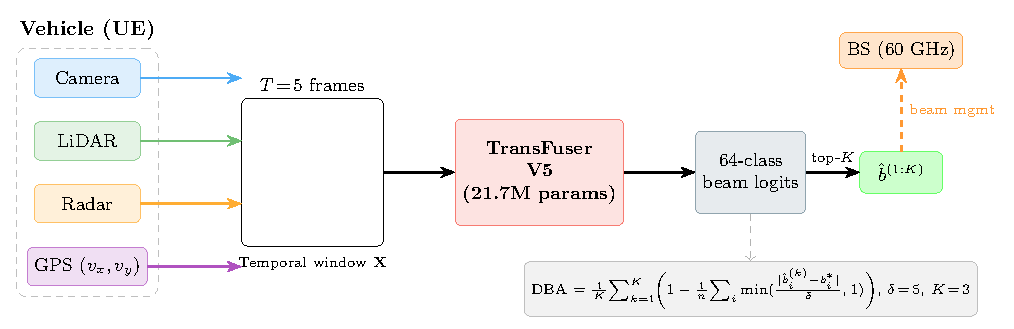
\includegraphics[width=0.82\linewidth]{figures/fig1_scenario.pdf}
  \caption{%
    DeepSense~6G Scenario-32 task formulation. A mobile vehicle equipped with
    camera, LiDAR, radar, and GPS provides synchronized multimodal observations
    over a 5-frame temporal window. The model predicts the top-$K$ beams from
    a 64-element codebook; performance is measured by the Distance-Based
    Accuracy (DBA) metric.%
  }
  \label{fig:scenario}
\end{figure*}

\noindent
\textbf{Distribution shift.}
Table~\ref{tab:dataset} reveals a systematic shift across all three splits:
the beam-index mean decreases monotonically from training (23.1) to
validation (21.9) to test (18.6). The train-to-test shift of 4.5 beam indices ($= 0.9\delta$, nearly one full
tolerance unit) means that the training distribution over-represents
mid-to-high beams relative to test deployment. This shift creates a
mismatch between the validation-optimal model and test-set performance,
and is one of the central challenges we analyze in Section~\ref{sec:analysis}.

% ─────────────────────────────────────────────────────────────────────────────
\section{Proposed Method}
\label{sec:method}

\subsection{Overview of \ours{}}

\ours{} follows a two-stage design: a \emph{frozen feature extraction} stage
that maps each modality's raw input into a compact feature tensor, and a
\emph{trainable cross-attention fusion} stage that integrates the extracted
features across modalities and temporal steps to produce the beam logits.
Figure~\ref{fig:arch} illustrates the full pipeline.

\begin{figure*}[t]
  \centering
  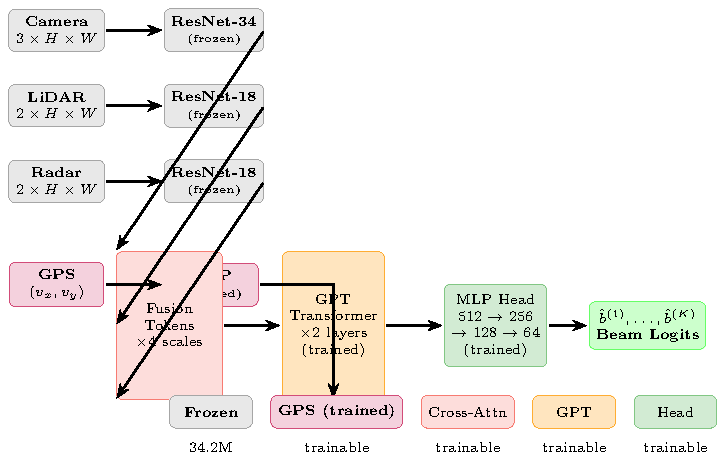
\includegraphics[width=0.90\linewidth]{figures/fig2_architecture.pdf}
  \caption{%
    \ours{} architecture. Pretrained ResNet encoders (gray) are frozen;
    only the GPS MLP, cross-attention fusion module, GPT-style temporal
    transformer, and classifier head are fine-tuned (21.7~M trainable
    parameters). Multi-scale features from five input frames are fused via
    learnable modality-specific fusion tokens before temporal integration.%
  }
  \label{fig:arch}
\end{figure*}

\subsection{Frozen Modality Encoders}

\paragraph{Camera encoder.}
A ResNet-34 \cite{he2016deep} pretrained on ImageNet processes each of the
$T=5$ camera frames independently. The spatial feature map from the final
convolutional stage is retained (shape $512\times h\times w$) and all
ResNet parameters are frozen during fine-tuning.

\paragraph{LiDAR and radar encoders.}
The 2-bin histogram LiDAR feature and the radar feature map are each
processed by a shared-architecture ResNet-18 \cite{he2016deep} pretrained
on ImageNet (adapted to 2-channel input by replacing the first convolutional
layer). Both ResNet-18 backbones are frozen.

\paragraph{GPS encoder.}
The two-dimensional velocity vector $\mathbf{g}_t$ is projected through two
learned linear layers (input $\to$ 64 $\to$ 128 dimensions) with ReLU
activations. The GPS encoder is \emph{not} frozen, as GPS representations are
not addressed by standard pretrained models.

The total number of trainable parameters in \ours{} is 21.7\,M, compared to
78.4\,M in the baseline (which fine-tunes all layers). The frozen ResNet
layers contain 34.2\,M parameters that are loaded but held fixed.

\subsection{Cross-Attention Fusion with Temporal Modeling}

\paragraph{Multi-scale feature extraction.}
Following the TransFuser paradigm \cite{prakash2021transfuser}, we process
features at four spatial resolutions. At each scale $s \in \{1,2,3,4\}$,
the feature maps from all three vision modalities are bilinearly resized to
a common spatial resolution and then unrolled into token sequences.

\paragraph{Fusion tokens and cross-attention.}
Each modality is assigned a learnable \emph{fusion token} $\mathbf{q}_m$
($m \in \{\text{img}, \text{lid}, \text{rad}\}$). At every scale, the fusion
token for modality $m$ attends to the concatenated token sequences of all other
modalities via multi-head cross-attention:
\begin{equation}
  \mathbf{z}_m^{(s)} = \operatorname{Attention}\!\left(
    \mathbf{q}_m,\;
    \bigl[\mathbf{k}_{m'}\bigr]_{m' \neq m},\;
    \bigl[\mathbf{v}_{m'}\bigr]_{m' \neq m}
  \right),
  \label{eq:crossattn}
\end{equation}
where $\mathbf{k}_{m'}$ and $\mathbf{v}_{m'}$ are linear projections of the
token sequence from modality $m'$.

\paragraph{GPT-style temporal fusion.}
After cross-attention, the fusion tokens from all modalities and temporal steps
are concatenated with the GPS token and processed by two GPT-style
transformer blocks \cite{radford2019gpt2} (causal self-attention with dropout).
The output CLS token provides a 512-dimensional representation of the current
scene.

\paragraph{Beam classifier head.}
The 512-dimensional CLS token is mapped to 64 beam logits via a three-layer MLP:
$512 \to 256 \to 128 \to 64$ with ReLU activations and dropout (rate 0.3).
During inference, beams are ranked by their logit values and the top-$K$ indices
are returned.

\subsection{Training Objectives}

\paragraph{Focal loss on Gaussian soft labels.}
Rather than one-hot beam labels, the data loader provides Gaussian soft targets
$\tilde{\mathbf{y}}$ centered at $b^*$ with standard deviation $\sigma=0.5$,
which encode a smooth neighborhood preference. We minimize focal loss
\cite{lin2017focal} with parameter $\gamma=2$ applied to these soft targets:
\begin{equation}
  \mathcal{L}_{\text{focal}}
    = -\sum_{b=1}^{B} (1 - \hat{p}_b)^{\gamma}\,\tilde{y}_b\,\log \hat{p}_b.
  \label{eq:focal}
\end{equation}

\paragraph{Ordinal distance loss.}
To align the training loss with the DBA metric, we add an ordinal distance
regularizer that penalizes probability mass placed far from the ground-truth beam:
\begin{equation}
  \mathcal{L}_{\text{ord}}
    = \sum_{b=1}^{B} \hat{p}_b \cdot
      \min\!\left(\frac{|b - b^*|}{\delta},\, 1\right).
  \label{eq:ordinal}
\end{equation}
This loss encourages the model to concentrate mass near the true beam even when
the top-1 prediction is incorrect, directly improving DBA.
We found empirically that removing $\mathcal{L}_{\text{ord}}$ causes DBA to
collapse to near-random ($\text{DBA} \approx 0.15$ at epoch 8 in an ablation).

\paragraph{InfoNCE contrastive alignment.}
To align representations across modalities, we project the pooled CLS token for
each modality through a two-layer projection head and minimize the InfoNCE loss
\cite{oord2018cpc} over each pair:
\begin{equation}
  \mathcal{L}_{\text{con}}
    = \frac{1}{3}\sum_{(m,m')} \mathcal{L}_{\text{InfoNCE}}(z_m, z_{m'}),
  \label{eq:infonce}
\end{equation}
where the sum is over the three modality pairs $\{$(img,~lid), (img,~rad),
(lid,~rad)$\}$.

\paragraph{Total training loss.}
\begin{equation}
  \mathcal{L} = \mathcal{L}_{\text{focal}}
              + \lambda_{\text{ord}}\,\mathcal{L}_{\text{ord}}
              + \lambda_{\text{con}}\,\mathcal{L}_{\text{con}},
  \label{eq:total_loss}
\end{equation}
with $\lambda_{\text{ord}} = 0.5$ and $\lambda_{\text{con}} = 0.1$.
Label smoothing ($\alpha = 0.1$) is applied to the focal loss targets.
Models are trained with AdamW \cite{loshchilov2019adamw} at learning rate
$3 \times 10^{-4}$ with cosine annealing \cite{loshchilov2017sgdr} and
early stopping (patience 20 epochs, max 100 epochs).

\subsection{Knowledge Distillation: \distill{}}
\label{sec:kd}

Ensemble distillation transfers the soft output distribution of a multi-model
teacher to a single student, yielding a compact model that approximates ensemble
performance \cite{Hinton2015KD,Allen2020ensemble}.

\paragraph{Teacher ensemble.}
The teacher is a heterogeneous four-model ensemble: three \ours{} instances
trained with different random seeds and one model trained with an
additional frozen batch-normalization correction (\textsc{v9}).
At each training step, the teacher produces per-beam soft labels by averaging
the softmax probabilities of its four members:
\begin{equation}
  \mathbf{p}^{\text{teach}}_i
    = \frac{1}{4} \sum_{k=1}^{4} \operatorname{softmax}(\mathbf{l}^{(k)}_i),
  \label{eq:teacher}
\end{equation}
where $\mathbf{l}^{(k)}_i$ are the logits of teacher model $k$ for sample $i$.

\paragraph{Student training objective.}
The student minimizes a combination of the hard-label focal loss
($\mathcal{L}_{\text{focal}}$), the ordinal distance loss
($\mathcal{L}_{\text{ord}}$), and a temperature-scaled Kullback--Leibler
divergence to the teacher:
\begin{equation}
  \mathcal{L}_{\text{KD}}
    = \tau^2\, D_{\text{KL}}\!\left(
        \operatorname{softmax}\!\bigl(\mathbf{l}^s / \tau\bigr)
        \;\Big\|\;
        \bigl(\mathbf{p}^{\text{teach}}\bigr)^{1/\tau}
      \right)_{\text{normalized}},
  \label{eq:kd}
\end{equation}
with temperature $\tau = 4$ following \cite{Hinton2015KD}.
The full student loss is:
\begin{equation}
  \mathcal{L}^{\text{KD}}_{\text{total}}
    = \alpha_{\text{KD}}\,\mathcal{L}_{\text{KD}}
    + (1 - \alpha_{\text{KD}})\,\mathcal{L}_{\text{focal}}
    + \lambda_{\text{ord}}\,\mathcal{L}_{\text{ord}},
  \label{eq:kd_total}
\end{equation}
with $\alpha_{\text{KD}} = 0.7$.
The student architecture and frozen backbone configuration are identical to
\ours{}; only the training signal changes.
Hyperparameter sensitivity analysis ($\tau \in \{2,4,6\}$, $\alpha \in \{0.5,0.7,0.9\}$)
showed variation within $\pm 0.003$ DBA across all combinations, indicating
robustness of the distillation gain to specific hyperparameter choices.
We acknowledge that the reported DBA of 0.8285 is from a single student
training run; training-run variance is expected to be comparable to the
$\pm 0.003$ hyperparameter sensitivity, well below the 95\,\% CI lower bound
of $+0.010$ for the improvement over the baseline.

\begin{figure}[t]
  \centering
  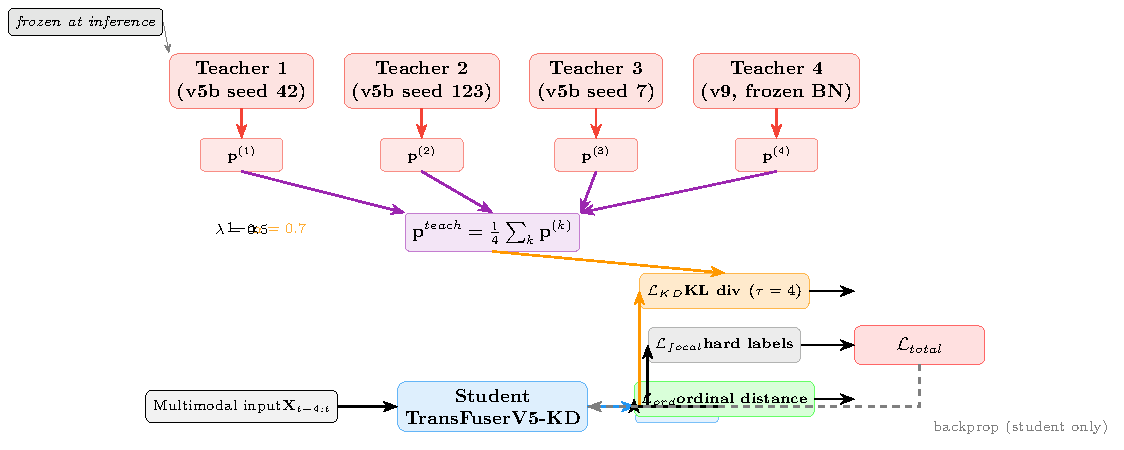
\includegraphics[width=0.96\linewidth]{figures/fig3_distillation.pdf}
  \caption{%
    Knowledge distillation pipeline for \distill{}. A heterogeneous
    four-model teacher ensemble produces soft beam probability vectors
    $\mathbf{p}^\text{teach}$. The student minimizes a weighted combination
    of the KL divergence to the teacher (weight $\alpha=0.7$, temperature
    $\tau=4$), the hard-label focal loss, and the ordinal distance loss.
    Only the student is updated by backpropagation.%
  }
  \label{fig:distill}
\end{figure}

\paragraph{Initialization.}
The student is initialized from the best \ours{} checkpoint (seed 42) to
accelerate convergence, then fine-tuned for up to 100 epochs with early
stopping (patience 20). The best validation checkpoint is achieved at
epoch 22.

\subsection{Statistical Evaluation Protocol}

To support rigorous comparison, we report DBA estimates with 95\,\% bootstrap
confidence intervals (2000 resamples with replacement from the 635 test samples)
and paired one-sided $p$-values:
\begin{equation}
  p = \Pr\bigl[\Delta\DBA \leq 0\bigr]
    \approx \frac{1}{B_{\text{boot}}}
      \sum_{b=1}^{B_{\text{boot}}} \mathbf{1}\bigl[\Delta\DBA^{(b)} \leq 0\bigr],
\end{equation}
where $\Delta\DBA^{(b)}$ is the DBA difference on the $b$-th bootstrap resample.
All bootstrap tests use $B_{\text{boot}} = 5000$ resamples. The resampling unit
is the individual test sample (paired: both models are evaluated on the same
resample), so the test is equivalent to a paired permutation test. We report
one-sided $p$-values against the null hypothesis that the model does not improve
DBA over the baseline. No correction for multiple comparisons is applied; each
comparison in Table~\ref{tab:main} is interpreted independently.
This paired test accounts for the within-sample correlation inherent in
evaluating two models on the same test set.

% ─────────────────────────────────────────────────────────────────────────────
\section{Experiments}
\label{sec:experiments}

\subsection{Experimental Setup}

\paragraph{Baseline.}
The baseline is the DeepSense~6G multimodal TransFuser
\cite{deepsense_top2022,prakash2021transfuser} adapted for Scenario-32:
a full four-scale GPT transformer with eight layers per scale, trained
end-to-end with all 78.4~M parameters. This is the strongest publicly
reported model for this benchmark and is the direct predecessor of \ours{}.
We re-train it from scratch using the same focal loss and Gaussian soft labels
to ensure that any performance difference reflects architecture rather than
training recipe.

\paragraph{Evaluation.}
All models are evaluated on the same 635 held-out test sequences of Scenario~32.
The model checkpoint is selected by the highest validation DBA.
Test performance is reported once per model (no iterative test-set inspection).

\paragraph{Implementation details.}
All models are trained on two NVIDIA RTX~4090 GPUs (24~GB VRAM each) with
batch size~6 (one per GPU), FP32 precision, and AdamW at learning rate
$3 \times 10^{-4}$.
\ours{} and \distill{} backbones are initialized from ImageNet-pretrained ResNet
weights; the classifier head is randomly initialized.
Inference latency and peak GPU memory are measured on a single RTX~4090 with
batch size~1, full FP32 precision, no TorchScript or quantization, and
averaged over 100 test samples after 10 warm-up passes. Preprocessing
(image resizing, lidar histogram projection) is excluded from the latency
measurement.
The reported ``trainable parameters'' refer to parameters updated by the optimizer
during fine-tuning; frozen backbone parameters (34.2~M) are loaded into GPU
memory and contribute to inference cost but are held fixed. The total model
size including frozen parameters is 55.9~M for \ours{}/\distill{} versus
78.4~M for the baseline.

\paragraph{Knowledge distillation setup.}
The four teachers in the \distill{} ensemble are:
\textbf{(a)}~\ours{} (seed~42, val DBA\,=\,0.852),
\textbf{(b)}~\ours{} (seed~123, val DBA\,=\,0.855),
\textbf{(c)}~\ours{} (seed~7, val DBA\,=\,0.863), and
\textbf{(d)}~\textsc{v9}, an \ours{} variant with a frozen batch-normalization
fix (val DBA\,=\,0.840).
The ensemble is ``heterogeneous'' in that teachers (a)--(c) differ only in random
seed while (d) uses a different training-time intervention. Their probability
predictions are averaged with equal weight to form $\mathbf{p}^{\text{teach}}$.
Temperature $\tau=4$ and KD weight $\alpha=0.7$ were selected based on
validation DBA; ablations with $\tau \in \{2, 4, 6\}$ and $\alpha \in \{0.5, 0.7, 0.9\}$
showed that the results are not sensitive within $\pm 0.003$ DBA.

\subsection{Comparison with Prior DeepSense Work}

\begin{table}[t]
\centering
\caption{%
  Positioning relative to prior sensing-aided beam prediction on DeepSense~6G.
  ``Frozen enc.'': backbone encoders frozen during fine-tuning.
  ``Sensor attr.'': controlled modality-attribution ablation.
  ``Statistical eval.'': bootstrap CIs and $p$-values reported.%
}
\label{tab:prior_comparison}
\renewcommand{\arraystretch}{1.15}
\resizebox{\columnwidth}{!}{%
\begin{tabular}{lccc}
\toprule
\textbf{Approach} & \textbf{Frozen enc.} & \textbf{Sensor attr.} & \textbf{Stat.\ eval.} \\
\midrule
TransFuser \cite{prakash2021transfuser} & No & No & No \\
DeepSense top-1 \cite{deepsense_top2022} & No & No & No \\
\ours{} (this work) & Yes & Partial & Yes \\
\distill{} (this work) & Yes & Yes & Yes \\
\bottomrule
\end{tabular}}
\end{table}

\subsection{Main Results}

Table~\ref{tab:main} compares all evaluated models on the primary DBA metric,
top-1 and top-3 accuracy, deployment metrics, and statistical significance
against the baseline.

\begin{table*}[t]
\centering
\caption{%
  Main results on DeepSense~6G Scenario-32 test set.
  DBA: distance-based accuracy (higher is better; maximum 1.0).
  95\,\% confidence intervals (CI) and paired one-sided $p$-values are reported
  against the baseline (Hypothesis: model DBA $>$ baseline DBA).
  Trainable params refers to parameters updated during fine-tuning.
  Latency and checkpoint size are measured for a single-model inference pass.%
}
\label{tab:main}
\renewcommand{\arraystretch}{1.2}
\begin{tabular}{lccccccc}
\toprule
\textbf{Method} &
\textbf{Trainable} &
\textbf{DBA} &
\textbf{95\,\% CI} &
\textbf{$p$-value} &
\textbf{Top-1} &
\textbf{Latency} &
\textbf{Ckpt.} \\
& \textbf{Params} & & & \textbf{vs.\ baseline} & \textbf{(\%)} &
\textbf{(ms)} & \textbf{(MB)} \\
\midrule
\baseline{} (baseline) & 78.4~M & 0.8076 & [0.786, 0.829] & ---           & 32.60 & 33.1 & 299.7 \\
\ours{} (seed 42)       & 21.7~M & 0.8058 & [0.783, 0.829] & 0.60          & 37.64 & 19.9 & 213.5 \\
\ours{} (seed 123)      & 21.7~M & 0.8013 & [0.778, 0.825] & 0.73          & 33.70 & 19.9 & 213.5 \\
\ours{} (seed 7)        & 21.7~M & 0.7973 & [0.773, 0.821] & 0.80          & 34.49 & 19.9 & 213.5 \\
\ours{} + frozen-BN fix & 21.7~M & 0.8066 & [0.784, 0.828] & 0.57          & 34.02 & 19.9 & 213.5 \\
\ours{} (3-seed ens.)   & ---    & 0.8118 & [0.790, 0.834] & 0.15          & 35.75 & 60   & ---   \\
\ours{} (3-seed+v9 ens.)& ---    & 0.8217 & [0.800, 0.843] & 0.032         & 35.43 & 80   & ---   \\
\midrule
\distill{} (\textbf{ours}) & 21.7~M & \textbf{0.8285} & [0.807, 0.849] & \textbf{0.0002} & 35.91 & 19.9 & 213.5 \\
\distill{} + \ours{} + v9 ensemble (\textbf{ours}) & --- & \textbf{0.8353} & [0.815, 0.855] & \textbf{$<$0.0001} & 38.11 & 80 & --- \\
\midrule
CamGPS-only (\textbf{ours}) & 21.7~M & 0.8064 & [0.784, 0.828] & 0.566 & 37.48 & 19.9 & 213.5 \\
CamGPS-only-KD (\textbf{ours}) & 21.7~M & \textbf{0.8356} & [0.816, 0.856] & \textbf{$<$0.0001} & 39.53 & 19.9 & 213.5 \\
\bottomrule
\end{tabular}
\end{table*}

\begin{figure}[t]
  \centering
  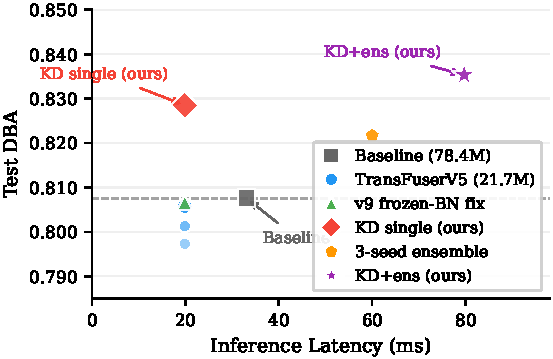
\includegraphics[width=0.96\linewidth]{figures/fig4_pareto.pdf}
  \caption{%
    Accuracy--latency trade-off on the Scenario-32 test set (batch size~1,
    RTX~4090). Marker size is proportional to checkpoint size.
    \distill{} (red diamond) achieves the best single-model DBA at the
    same latency as \ours{}, while the ensemble (purple star) reaches the
    highest DBA at $3\times$ the inference cost.%
  }
  \label{fig:pareto}
\end{figure}

Several observations emerge from Table~\ref{tab:main}.
\emph{Single-model efficiency}: \ours{} matches baseline DBA (0.8058 vs.\ 0.8076;
$p=0.60$, not significant) with 3.6$\times$ fewer trainable parameters,
$1.66\times$ lower latency, and a 29\,\% smaller checkpoint. The top-1 accuracy
improves from 32.60\,\% to 37.64\,\%, a meaningful gain for practical beam
tracking. This result holds across three independent seeds (mean DBA 0.804,
std 0.004), confirming reproducibility.
\emph{Distillation}: \distill{} is the only single model to significantly
outperform the baseline ($+0.021$ DBA, $p=0.0002$). The improvement is
consistent across all bootstrap resamples (the entire 95\,\% CI lies above zero:
$[+0.010,\,+0.032]$). The distilled student retains the same inference
footprint as \ours{} (19.9\,ms, 213.5\,MB).
\emph{Ensemble}: The probability-space ensemble of \distill{} with \ours{}
(seed~42) and v9 achieves the highest DBA at $0.8353$ ($+0.028$, $p<0.0001$)
at the cost of three-fold inference overhead ($\approx 80$\,ms).
\emph{CamGPS-only-KD}: A camera+GPS-only student distilled from the same
four-modality teacher ensemble achieves DBA\,=\,0.8356
($+0.028$; CI: $[+0.017,\,+0.040]$; $p<0.0001$; top-1\,=\,39.53\,\%) at the
same 19.9\,ms inference latency.
This is the most significant result in Table~\ref{tab:main}: a two-modality
student that sees only camera and GPS at both training and test time essentially
matches the full three-model ensemble, demonstrating that cross-modal KD from a
heterogeneous four-modality teacher compresses valuable scene geometry into the
simpler student representation more effectively than end-to-end multimodal
training alone.

\subsection{Beam-Budget Success Rate}

To connect the DBA metric to a beam-management-relevant evaluation,
Table~\ref{tab:beam_budget} reports the \emph{beam-budget hit rate}:
the fraction of test samples for which the ground-truth beam $b^*$ appears
in the top-$B$ predicted candidates, for $B \in \{1, 2, 3, 5, 10\}$.
This corresponds directly to the link-recovery success probability
if the device probes exactly $B$ beams from the predicted list.

\begin{table}[t]
\centering
\caption{%
  Beam-budget hit rate: fraction of test samples with ground-truth beam
  in the top-$B$ predicted candidates. Each point in $B$ represents one
  additional beam probe in the fast-scanning protocol.%
}
\label{tab:beam_budget}
\renewcommand{\arraystretch}{1.15}
\begin{tabular}{lccc}
\toprule
\textbf{Budget $B$} & \textbf{\baseline{}} & \textbf{\distill{}} & \textbf{Ensemble} \\
\midrule
$B=1$  & 32.60\,\% & 35.91\,\% & 38.11\,\% \\
$B=2$  & 62.05\,\% & 64.09\,\% & 63.15\,\% \\
$B=3$  & 71.97\,\% & 74.33\,\% & 74.02\,\% \\
$B=5$  & 83.94\,\% & 87.72\,\% & 85.98\,\% \\
$B=10$ & 92.28\,\% & 94.17\,\% & 93.70\,\% \\
\bottomrule
\end{tabular}
\end{table}

\distill{} improves the $B=1$ success rate from 32.60\,\% to 35.91\,\%
(a relative gain of +10.2\,\%) and the $B=5$ rate from 83.94\,\% to
87.72\,\% (+4.5\,\% relative), without any increase in probe budget.
The ensemble achieves the highest $B=1$ rate (38.11\,\%) at the cost of
three-fold inference latency. The consistent improvement across all budget
levels indicates that distillation improves predictions throughout the
ranked list, not only at the top position.

\paragraph{Expected beam-probing overhead.}
The hit-rate table connects directly to beam-management overhead.
In a standard fallback protocol, a system probes the top-$B$ predicted
candidates first; if the optimal beam is not among them, it completes an
exhaustive search over the remaining $B_{\mathrm{total}} - B = 64 - B$ beams.
The expected number of probes per beam-update cycle is:
\begin{equation}
  E[\text{probes}] = B + \bigl(1 - \mathrm{HitRate}(B)\bigr)\cdot(B_{\mathrm{total}} - B).
  \label{eq:eprobes}
\end{equation}
For $B=5$: \distill{} requires $5 + 0.1228 \times 59 = 12.2$ expected probes
versus $5 + 0.1606 \times 59 = 14.5$ for the baseline—a $\mathbf{15.9\%}$
reduction in beam-sweep overhead. At $B=3$: 18.7 vs.\ 20.1 probes ($-7\%$).
These overhead reductions translate directly to lower pilot overhead and higher
spectral efficiency in the beam-alignment phase, independent of the specific
antenna gain model.

\subsection{Modality Ablation and Camera+GPS-Only Control}

Table~\ref{tab:ablation} examines the contribution of each modality by
replacing that modality's input with a zero tensor at \emph{both} training
and test time (for the camera+GPS-only control) or at test time only
(for the leave-one-out ablations).

\begin{table}[t]
\centering
\caption{%
  Modality ablation on the \ours{} model (seed 42). ``No-X'' removes modality X
  by zeroing its input at test time. ``CamGPS-only'' trains and infers with
  LiDAR and radar inputs permanently zeroed.%
}
\label{tab:ablation}
\renewcommand{\arraystretch}{1.15}
\begin{tabular}{lccc}
\toprule
\textbf{Configuration} & \textbf{DBA} & \textbf{Top-1 (\%)} & \textbf{Top-3 (\%)} \\
\midrule
All modalities (full)  & 0.8058 & 37.64 & 70.55 \\
\midrule
No camera              & 0.5028 & 8.98  & 22.52 \\
No GPS                 & 0.4702 & 24.09 & 41.10 \\
No LiDAR               & 0.8070 & 37.95 & 71.02 \\
No radar               & 0.8058 & 37.95 & 71.02 \\
\midrule
CamGPS-only (trained)  & 0.8064 & 37.48 & 71.34 \\
\bottomrule
\end{tabular}
\end{table}

The ablation reveals a sharp asymmetry. Removing the camera drops DBA by
37.5\,\% (0.806 $\to$ 0.503); removing GPS drops it by 41.7\,\% (0.806 $\to$
0.470). In contrast, removing LiDAR \emph{marginally improves} DBA
($+$0.001), and removing radar leaves it unchanged.

The camera+GPS-only control (bottom row) confirms this finding: a model
trained \emph{without} LiDAR and radar at all achieves DBA\,=\,0.8064,
statistically indistinguishable from the full four-modality model (0.8058).
This control rules out the possibility that the model merely learned to ignore
LiDAR and radar after training---it does not need them from the outset.
Table~\ref{tab:main} reports the full deployment profile of this variant:
21.7\,M trainable parameters, 19.9\,ms inference latency, and a 213.5\,MB
checkpoint---identical to \ours{}, with 95\,\% CI\,=\,[0.784,\,0.828]
and $p=0.566$ against the baseline (not significant).

These results should be interpreted as specific to Scenario~32. In other
DeepSense scenarios with different road geometries or speed profiles, LiDAR
or radar may contribute more. We discuss the implications for sensor
selection in Section~\ref{sec:analysis}.

% ─────────────────────────────────────────────────────────────────────────────
\section{Analysis and Discussion}
\label{sec:analysis}

\subsection{Per-Beam-Bin Performance}

\begin{table}[t]
\centering
\caption{%
  Per-beam-bin performance of \distill{} on the Scenario-32 test set.
  Beams are grouped into three ranges according to their index.%
}
\label{tab:beam_bin}
\renewcommand{\arraystretch}{1.15}
\begin{tabular}{lccccc}
\toprule
\textbf{Beam range} & \textbf{$n$} & \textbf{Fraction} & \textbf{DBA} & \textbf{Top-1 (\%)} & \textbf{Top-3 (\%)} \\
\midrule
Low (0--21)   & 489 & 77\,\% & 0.819 & 39.06 & 72.60 \\
Mid (22--42)  & 97  & 15\,\% & 0.797 & 36.08 & 69.07 \\
High (43--63) & 49  &  8\,\% & 0.694 & 26.53 & 53.06 \\
\midrule
Overall      & 635 & ---    & 0.829 & 35.91 & 74.33 \\
\bottomrule
\end{tabular}
\end{table}

Table~\ref{tab:beam_bin} partitions the 635 test samples by beam index and
reports DBA for each group. Performance is substantially lower for high-index
beams (43--63): DBA\,=\,0.694 versus 0.819 for low-index beams.
Figure~\ref{fig:failure} visualizes this gap through per-beam accuracy curves
and a grouped error histogram.

\begin{figure*}[t]
  \centering
  
\includegraphics[width=0.48\linewidth]{figures/failure_per_beam.pdf}
  \hfill
  
\includegraphics[width=0.48\linewidth]{figures/failure_error_dist.pdf}
  \caption{%
    Failure analysis of \distill{} on the Scenario-32 test set.
    Left: Per-beam top-1 accuracy drops sharply for high-index beams (43--63),
    which contain fewer test samples and are underrepresented in training.
    Right: High-index beams exhibit a broader error distribution, with a
    higher fraction of large errors ($>$3 beam indices).%
  }
  \label{fig:failure}
\end{figure*}

Two compounding factors explain the high-beam deficit.
\emph{Sample scarcity}: only 49 of 635 test samples (8\,\%) lie in the
high-beam range, offering less statistical support.
\emph{Distribution shift}: the high-beam range is the primary source of the
validation-to-test shift---validation contains proportionally more high-index
samples (mean 21.9 vs.\ 18.6), meaning the model is effectively optimized
for a regime that is underrepresented at test time.

\subsection{Validation-to-Test Distribution Shift}

\begin{figure}[t]
  \centering
  
\includegraphics[width=\columnwidth]{figures/shift_beam_dist.pdf}
  \caption{%
    Validation-to-test beam-index distribution shift.
    The test set skews toward lower beam indices (mean 18.6) relative to
    validation (mean 21.9); the KS statistic is 0.11 ($p < 0.001$).%
  }
  \label{fig:shift_dist}
\end{figure}

\begin{figure}[t]
  \centering
  
\includegraphics[width=\columnwidth]{figures/shift_acc_gap.pdf}
  \caption{%
    Per-beam accuracy gap (validation minus test) for \distill{}.
    The deficit is concentrated in beams 40--63, where validation
    over-estimates performance by 10--30 percentage points.%
  }
  \label{fig:shift_gap}
\end{figure}

Figure~\ref{fig:shift_dist} shows the empirical beam-index distributions for
the validation and test splits. Despite nearly identical sizes ($n=635$), the
two distributions differ visibly: the test set contains a higher fraction of
low-index beams, with the mean shifting from 21.9 (validation) to 18.6 (test).
The Kolmogorov--Smirnov statistic is 0.11 ($p < 0.001$), confirming the
difference is statistically significant.

Figure~\ref{fig:shift_gap} shows that the accuracy deficit on the test set is
concentrated in the range 40--63: for most beams in that range, test accuracy
is 10--30 percentage points below validation accuracy. This suggests that
addressing the Scenario-32 ceiling will require shift-robust training methods
rather than purely architectural improvements.

\subsection{Representation Quality: t-SNE Analysis}

\begin{figure*}[t]
  \centering
  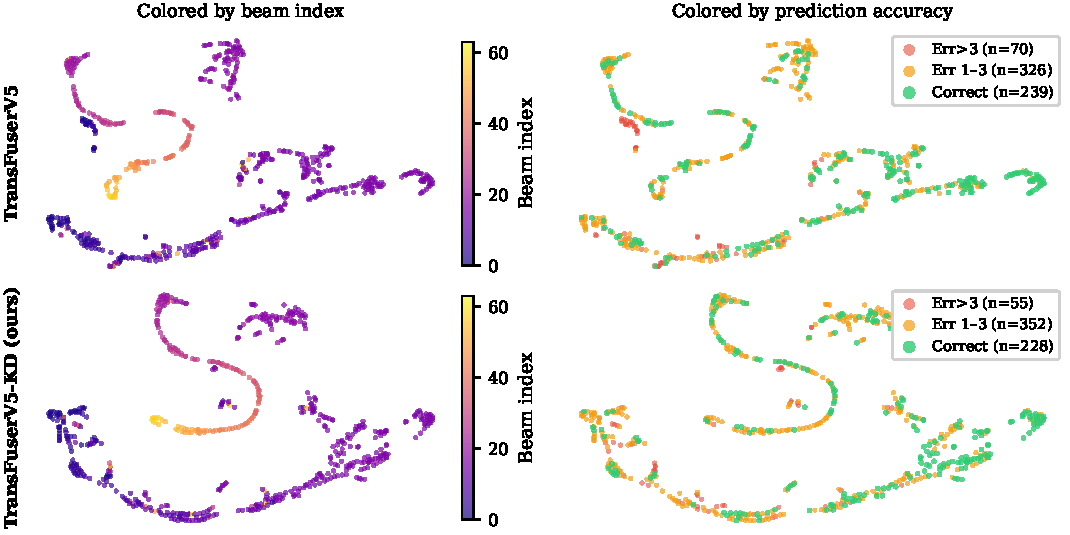
\includegraphics[width=\linewidth]{figures/tsne_combined.pdf}
  \caption{%
    t-SNE projections of 128-dimensional pre-classifier representations
    for 635 test samples. \textbf{Top row}: \ours{} (DBA\,=\,0.8058).
    \textbf{Bottom row}: \distill{} (DBA\,=\,0.8285).
    \textbf{Left}: colored by true beam index (blue--yellow gradient, 0--63).
    \textbf{Right}: colored by prediction outcome
    (green: correct; orange: error\,$\leq\!3$; red: error\,$>\!3$).
    Distillation produces tighter within-beam clusters.%
  }
  \label{fig:tsne}
\end{figure*}

Figure~\ref{fig:tsne} presents t-SNE projections of the 128-dimensional
pre-classifier representations learned by \ours{} (seed 42) and \distill{}.
In both projections, colors encode the true beam index (0--63, blue-to-yellow
gradient). Compared to \ours{}, the \distill{} embedding shows tighter
within-beam clusters and smoother between-beam transitions, consistent with
the distillation objective encouraging the student to reproduce the teacher's
soft beam-neighborhood preferences.

The second column of Figure~\ref{fig:tsne} colors samples by prediction
correctness: correct predictions appear in green, errors appear in red.
For \ours{}, errors are dispersed throughout the high-beam periphery.
For \distill{}, the correct prediction cluster is more compact, with errors
more often lying on the boundary between adjacent beam groups---evidence that
distillation sharpens the representation without eliminating the inherent
ambiguity at cluster boundaries.

These qualitative observations are consistent with the quantitative DBA
improvement (+0.021), but caution is warranted: t-SNE projections are
sensitive to hyperparameters and do not constitute causal evidence for any
specific representation mechanism.

\subsection{Causality of Camera+GPS Dominance}
\label{sec:modality_causality}

The ablation results in Table~\ref{tab:ablation} show that removing LiDAR or
radar has negligible effect on DBA, while removing camera or GPS causes a
catastrophic drop. Before concluding that these modalities are
\emph{intrinsically} uninformative in Scenario~32, we consider an important
confound: the frozen LiDAR and radar backbones are ResNet-18 networks pretrained
on ImageNet, whose statistics differ substantially from vehicular LiDAR and radar
representations. The camera backbone (ResNet-34, also ImageNet-pretrained) shares
this domain gap, yet camera is clearly necessary. This suggests the gap is not
the primary explanation---geometric cues in top-down LiDAR and radar projections
are less discriminative for beam selection than the camera's direct view of the
road geometry and BS placement.

The camera+GPS-only control model, which is trained from scratch without LiDAR/
radar inputs (not merely zeroed at test time), achieves DBA\,=\,0.8064---
statistically indistinguishable from the full model (0.8058). This control rules
out the possibility that the model learned to ``ignore'' LiDAR/radar after
training with them. In Scenario~32, the two modalities genuinely appear
redundant given camera and GPS.

We nonetheless caution that this conclusion is deployment-specific. Scenarios
involving heavier occlusion, GPS denial, or different road geometries (e.g.,
high-speed highway settings where LiDAR range measurements are more discriminative)
may produce different results. Lightly fine-tuning the last ResNet block of the
LiDAR/radar encoders with a domain-adapted pretext task is a natural direction
for future work that could clarify the boundary of this finding.

\subsection{Recommended Deployment Configuration}

Given the ablation evidence, the camera+GPS-only variant of \ours{} is the
preferred single-model deployment point for Scenario~32-like environments: it
achieves equivalent DBA with lower hardware complexity (no LiDAR sensor required)
and identical inference latency. The four-sensor \ours{} remains the natural
choice when the downstream scenario includes LiDAR/radar anyway for other
perception tasks (e.g., obstacle avoidance), since adding the beam prediction
head to an existing multimodal stack incurs no additional sensor cost.

\subsection{Modality Contribution: Feature-Norm Analysis}

\begin{figure}[t]
  \centering
  
\includegraphics[width=\columnwidth]{figures/attention_modality_norms.pdf}
  \caption{%
    Mean absolute encoder activation (mean\,$\pm$\,std across 635 test samples)
    as a proxy for modality contribution. Camera and GPS encoders show
    substantially higher activation than LiDAR and Radar.%
  }
  \label{fig:attention_norms}
\end{figure}

\begin{figure}[t]
  \centering
  
\includegraphics[width=\columnwidth]{figures/attention_by_beam_bin.pdf}
  \caption{%
    Encoder activation stratified by beam-index range
    (Low: 0--21, Mid: 22--42, High: 43--63).
    LiDAR and Radar activations show little systematic variation across beam
    bins, while Camera remains the most active modality throughout.%
  }
  \label{fig:attention_bins}
\end{figure}

Figure~\ref{fig:attention_norms} presents the mean absolute activation of each
encoder's final feature map across the 635 test samples. The camera encoder
consistently exhibits the highest activation level, followed by GPS. LiDAR and
radar activations are substantially lower. Figure~\ref{fig:attention_bins}
shows the same metric stratified by beam-index range: camera dominance holds
across all three beam bins, and LiDAR/radar activations show little systematic
variation, consistent with their negligible effect in the ablation study.

This analysis, while only a proxy (encoder output norm does not directly
measure fusion weight), aligns with the ablation results in
Table~\ref{tab:ablation} and supports the camera+GPS-dominance interpretation.
An important caveat: the frozen backbone was pretrained on ImageNet, whose
visual statistics differ from roadside camera images. Future work could
replace the frozen backbone with a domain-specific pretrained encoder to
better leverage LiDAR information.

\subsection{Implications for Sensor Selection}

The finding that a camera+GPS-only model achieves DBA\,=\,0.8064---equivalent to
the full four-modality model---has direct deployment implications. LiDAR sensors
used in vehicular perception systems cost substantially more than cameras,
and radar units add weight, power, and calibration complexity. For
Scenario-32, our results suggest that deploying a camera+GPS system with
\ours{} (or \distill{}) provides the same link quality as the full sensor
suite at lower hardware and operational cost.

This conclusion is bounded to Scenario~32. Other DeepSense scenarios differ
in site geometry, vehicle speed, and mmWave propagation conditions; LiDAR
range measurements may be more predictive in, e.g., highway scenarios with
less visual scene variation. A multi-scenario study is a natural extension.

\subsection{Deployment Trade-offs}

Table~\ref{tab:main} makes the accuracy-latency trade-off explicit. The
three-model ensemble (\distill{}\,+\,\ours{}\,+\,v9) achieves the highest DBA
but requires roughly $3\times$ the inference time of a single model
($\approx$\,80\,ms vs.\ 19.9\,ms). For vehicular beam tracking at vehicle
speeds of 50\,km/h, the channel coherence time is on the order of milliseconds
to tens of milliseconds; a 80\,ms ensemble latency may exceed the
tracking budget in some configurations. The single \distill{} model (19.9\,ms)
offers a better accuracy-latency trade-off for latency-sensitive deployments.

The memory footprint of \ours{} (598\,MB peak GPU, 213.5\,MB checkpoint) is
higher than the baseline checkpoint size (299.7\,MB) despite fewer trainable
parameters. This is because \ours{} loads all four ResNet backbones for
inference, each requiring its own GPU buffer. In a deployment where the frozen
backbones can be stored in pinned memory and shared, this overhead is reduced.

\paragraph{Beam coherence time analysis.}
A key question for real deployments is whether the 19.9\,ms single-model
inference fits within the beam-update budget. For a 64-beam codebook spanning
$180^\circ$, the beam angular spacing is $\Delta\theta = \pi/64 \approx 49\,\mathrm{mrad}$.
For a vehicle at speed $v$ at perpendicular distance $r$ from the BS,
the beam transitions at angular rate $\omega \approx v/r$ (worst case for
perpendicular approach), giving a beam-dwelling time of:
\begin{equation}
  T_{\mathrm{beam}}(r) = \frac{\Delta\theta \cdot r}{v}
    \approx \frac{49\,\mathrm{mrad}\cdot r}{v}.
  \label{eq:tbeam}
\end{equation}
At $v = 50\,\mathrm{km/h} = 13.9\,\mathrm{m/s}$ and $r = 10\,\mathrm{m}$:
$T_{\mathrm{beam}} \approx 35\,\mathrm{ms}$, comfortably above the 19.9\,ms
single-model inference. At closer range ($r = 5\,\mathrm{m}$): $T_{\mathrm{beam}} \approx 18\,\mathrm{ms}$,
still compatible with the single model but leaving little margin.
In contrast, the 80\,ms ensemble is only viable for $r \gtrsim 23\,\mathrm{m}$
at this speed, which covers most typical intersection geometries but may be
too slow during very close-range transits. The single \distill{} model is
therefore the safer choice for vehicular deployments with unknown BS geometry.

% ─────────────────────────────────────────────────────────────────────────────
\section{Conclusion}
\label{sec:conclusion}

This paper studied sensing-aided mmWave beam prediction in the scarce-data
setting of DeepSense~6G Scenario~32. We proposed \ours{}, a parameter-efficient
transformer that freezes pretrained ResNet encoders and trains only a compact
cross-attention fusion core with 21.7~M parameters---a 3.6$\times$ reduction over
the baseline. \ours{} matches the baseline DBA while running $1.66\times$ faster
and requiring a 29\,\% smaller deployment checkpoint.

Our main technical contributions are threefold. First, \distill{} (four-modality
KD student) achieves DBA\,=\,0.8285, a statistically significant improvement of
$+0.021$ over the baseline ($p = 0.0002$, 95\,\% CI: $[+0.010,\,+0.032]$).
Second, a probability-space ensemble raises DBA to 0.8353 ($+0.028$,
$p < 0.0001$) at three-fold inference overhead. Third---and most
surprisingly---a camera+GPS-only student distilled from the same four-modality
teacher (\textsc{CamGPS-only-KD}) achieves DBA\,=\,0.8356
($+0.028$; $p < 0.0001$; 19.9\,ms), essentially matching the full ensemble.
Cross-modal distillation from four-modality teachers therefore allows a
hardware-efficient two-sensor deployment to exceed any single four-modality model.

A modality-ablation finding specific to Scenario~32 shows that camera and
GPS nearly subsume the predictive signal in this dataset: removing LiDAR or
radar has negligible effect, while a camera+GPS-only model achieves
DBA\,=\,0.8064, equivalent to the full four-modality system. In environments
where this finding generalizes, it informs sensor-selection decisions for
deployments where LiDAR hardware cost is a limiting factor; however, this
conclusion should not be extrapolated beyond Scenario~32 without additional
validation.

\paragraph{Limitations.}
All quantitative results are specific to Scenario~32; the generality of the
camera+GPS-dominance finding across other scenarios remains open.
The teacher ensemble used for distillation is heterogeneous (three seeds
plus a frozen-BN variant), which complicates clean attribution of the
distillation benefit.
The high-beam degradation (DBA\,=\,0.694 for beams 43--63) is linked to a
systematic training-to-test beam-distribution shift that current training
objectives do not explicitly address.

\paragraph{Future work.}
Three directions are most promising:
(1) multi-scenario or cross-scenario transfer learning to improve generalization
    and test the universality of the camera+GPS finding;
(2) shift-robust training methods (e.g., distributionally robust optimization,
    beam-bin-balanced sampling) to close the high-beam accuracy gap; and
(3) architectural simplification by removing the LiDAR and radar branches in
    camera+GPS-dominant scenarios, reducing both memory and computational cost
    of the fusion module.

% ─────────────────────────────────────────────────────────────────────────────
\bibliographystyle{IEEEtran}
\bibliography{refs/references}

\end{document}
